\section{Mapping} 

This section describes the mapping concept used in this thesis. The mapping puts together the data gathered by the sensors and the results of the visual data extraction into a semantic map. In addition to the information about drivable space and obstacles needed for navigation the semantic map also contains information about rooms, room types and objects to enable an intelligent search planning.  %TODO better word for visual data extraction

The first main idea is to use a hybrid map. The chosen hybrid map design combines two paradigms, grid-based and topological. Grid-based maps are accurate metric maps ideal for navigation. However, with increasing size grid-based maps are difficult to keep consistent and the efficiency goes down, especially for movement planning. Topological maps on the other hand are more difficult to use for local navigation, but scale very well. A hybrid map can combine the benefits of both map types. Indoor environments are very suitable for such a hybrid map. On a higher level an indoor environment can be represented by a topology of rooms and every room can then be described separately in more detail using a grid-based map. Therefore this approach was used in this work. Every discovered room gets its own grid-based metric map, not only containing occupancy information but also information about the types of areas in the room and object locations. Each room is also a node in the high-level topological map capturing the room structure of the environment. Another benefit of this design is the possibility to split the search problem into two abstraction levels, which will be described later in this chapter.
 
The second main idea is to use a 2D simultaneous localization and
mapping (SLAM) system based on a Rao-Blackwellized particle filter. 

SLAM is a difficult problem as the quality of the map depends on the quality of the localization and vice versa. This leads to uncertainty in the map, the current pose and also the whole path. This uncertainty has to be taken into account when information is added to the map. The easiest way to do this is probably using a SLAM systems based on a Rao-Blackwellized particle filter. In this approach uncertainty is represented by particles and their weights. The particle itself has no uncertainty. Therefore all other maps can be created with known pose. The drawback of this approach is that every particle needs its own set of maps, making it only feasible for low particle numbers. To overcome this drawback sophisticated sampling techniques, like the one used in Gmapping, can be used, which allow to create high-quality maps even with low particle numbers. The maps of the currently most likely particle are then used in the other parts of the system. 2D SLAM was chosen over 3D SLAM as tests using 3D SLAM systems showed mediocre results, probably because of the inaccuracy and unreliability of the RGBD-camera compared to the LIDAR.  %TODO Gmapping reference?

The map representation consists of a topological map with a node for every room and an edge for every doorway connecting two rooms. Each room has a set of maps, called semantic room map, containing different information for every particle. These are:
\begin{itemize}
 \item Two 2D occupancy grid maps: One is created by the SLAM system based on the range measurements of the LIDAR and used for localization. The second one is based on the first 2D map, but also contains the obstacles detected by 3D mapping and is used for navigation, exploration and in-room search planning.
 \item A 3D occupancy grid map: This map is created using the RGBD-camera. It is used in the creation of the 2D occupancy grid map for navigation and also in the calculation of likely object locations.
 \item A Room-Type-Map: This is a 2D grid map, where every grid cell contains a probability distribution over all detectable room types. It is created using the results of the room type classification.
 \item An Object-Map for every detectable object class: These are 61 3D grid maps containing the probability of an object of the corresponding type being seen in a grid cell given the cell is occupied. These maps are created based on the result of the object detection.
 \item An Object-Probability-Map: This is a 3D grid map containing the probability of the currently searched object being in a grid cell. This map is only created for the currently most likely particle and the searched object type. It is created out of the information in the other maps and the commonsense knowledge.
\end{itemize}

Furthermore, the semantic room map contains estimated locations of detected doorways. 

In the following subsections the individual parts of the mapping system are presented in more detail. The generation of the high-level attributes of the room, like the total object probability and the expected search time, is described at the end of this section.

\subsection{3D Mapping and Creation of the 2D Map for Navigation }

3D mapping is done using the OctoMap library, which does 3D mapping with known pose using an Octree representation for the map. Each node in the Octree represents a cube in space and contains a probability value for being occupied. These probabilities are later used in the creation of the Object-Probability-Map. As some obstacles, like tables, are not sufficiently detectable by the LIDAR, the information in the 3D map is also necessary for safe navigation. To avoid the more complex path planning in 3D this additional information about obstacles is inserted into a second 2D map, which is then used for navigation. Therefore all nodes in the Octomap with an occupancy probability higher than a threshold and a smaller z-coordinate than the robots height are projected into the 2D map. This is illustrated in Figure \ref{fig:downproj}. %TODO: OctoMap reference?

\begin{figure}[h]
\centering
  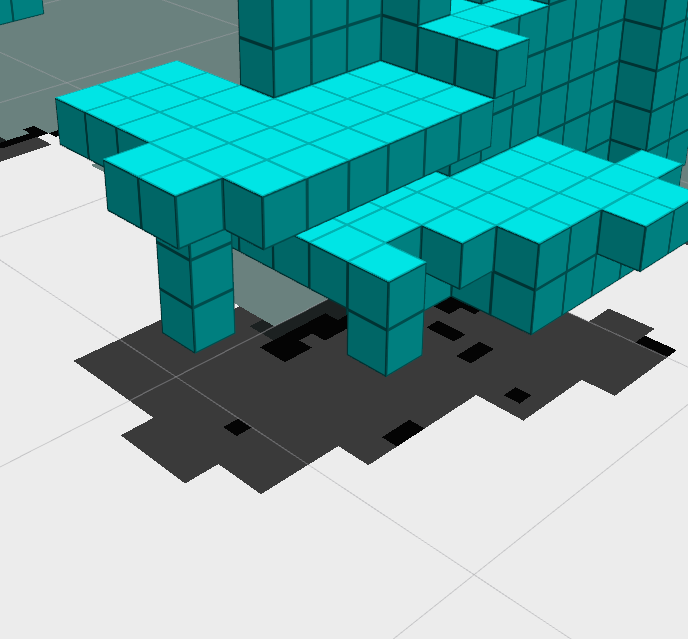
\includegraphics[width=0.5\textwidth]{figures/downproj.png}
  \caption[Downprojection of obstacles in the 3D map]{A snippet of a room showing a table and chairs, which are insufficiently detected by the LIDAR: 3D map (teal) and 2D map are shown; the light area is free, the black cells are obstacles in the 2D map and the dark gray cells are set occupied by the down-projection procedure}
  \label{fig:downproj}
\end{figure}

\subsection{Object-Map Creation} %TODO: better name?
\label{sec:Object Mapping}

This section covers the creation of the Object-Map, which contains information about the positions of the objects seen by the robot. The object detection can detect lots of objects in an image, especially in cluttered indoor environments. Those detections are often not very reliable and the location and especially the extent of the detected objects is inaccurate. All together an object tracking approach is not very promising. Therefore a grid map representation containing object probabilities was chosen. This approach can handle uncertainty much better and the number of detected objects has no impact on the performance.

For every detectable object class an independent 3D grid map is created. Every cell in this grid map holds the probability of containing an object of the corresponding type given it is occupied. Mapping this conditional probability is beneficial, as the result of the object detection are sample points, which lie on object surfaces and therefore in occupied cells, assuming the depth measurements are accurate. The unconditional probability can be calculated using the 3D occupancy map. With this approach the costly ray-tracing, which is necessary to find the cells to be marked as free, has only to be done in the 3D mapping.

Some assumptions were made to make this problem feasible. Independence of the grid cells and a static map are assumed. These are assumptions regularly made in similar problems, like occupancy grid mapping. Another assumption is the independence of different object types. This assumption implies that multiple objects can be located in a grid cell. This is reasonable if the resolution of the grid is not very high, which is the case. 

Using those assumptions and Bayes' theorem the following formula can be derived: 
\begin{multline}
 P(O_{c}^{o}|I_{1:t}, \mathbf{x}_{1:t},occ_{c}) = \\ 
 \frac{P(O_{c}^{o}|I_{t}, \mathbf{x}_{t},occ_{c})P(I_{t}| \mathbf{x}_{t},occ_{c})P(O_{c}^{o}|I_{1:t-1}, \mathbf{x}_{1:t-1},occ_{c})}
 {P(O_{c}^{o}|occ_{c})P(I_{t}|I_{1:t-1}, \mathbf{x}_{1:t},occ_{c})} 
 = \\ \frac{1}{Z} \frac{P(O_{c}^{o}|I_{t}, \mathbf{x}_{t},occ_{c})P(O_{c}^{o}|I_{1:t-1}, \mathbf{x}_{1:t-1},occ_{c})}
 {P(O_{c}^{o}|occ_{c})}
\end{multline}
$P(O_{c}^{o}|I_{1:t}, \mathbf{x}_{1:t},occ_{c})$ is the probability of cell $c$ containing an object of type $o$ given the RGBD-images $I_{1:t}$, the poses these images were taken at $\mathbf{x}_{1:t}$ and being occupied. $P(O_{c}^{o}|I_{t}, \mathbf{x}_{t},occ_{c})$ is the inverse sensor model, $P(O_{c}^{o}|I_{1:t-1}, \mathbf{x}_{1:t-1},occ_{c})$ is the recursive term and $P(O_{c}^{o}|occ_{c})$ is the prior. $Z$ is a normalization term, which can also be calculated by: 
\begin{multline}
 Z=\frac{P(O_{c}^{o}|I_{t}, \mathbf{x}_{t},occ_{c})P(O_{c}^{o}|I_{1:t-1}, \mathbf{x}_{1:t-1},occ_{c})}{P(O_{c}^{o}|occ_{c})}+\\ \frac{P(\neg O_{c}^{o}|I_{t}, \mathbf{x}_{t},occ_{c})P(\neg O_{c}^{o}|I_{1:t-1}, \mathbf{x}_{1:t-1},occ_{c})}{P(\neg O_{occ,c}^{OT}|occ_{c})}
\end{multline}
as the sum of $P(O_{c}^{o}|I_{1:t}, \mathbf{x}_{1:t},occ_{c})$ and $P(\neg O_{c}^{o}|I_{1:t}, \mathbf{x}_{1:t},occ_{c})$ has to be one. 

In this problem the prior cannot be set to $0.5$ as an occupied cell usually does not contain an object of a certain object type. Furthermore a low prior probability is necessary for many very uncertain object detections, resulting in a high object probability, which is an intended behavior. The value of the prior had to be estimated empirically.

Finding a suitable inverse sensor model is a difficult task, as it has to cope with the uncertain results of the object detection and other detectable or not detectable objects in the cell.

The chosen inverse sensor model is
\begin{equation}
 P(O_{c}^{o}|I_{t}, \mathbf{x}_{t},occ_{c})=\begin{cases}\max_{s \in \mathbf{S_t^c}} V_{hit}P(O_{s}^{o}|I_t)+V_{miss}(1-P(O_{s}^{o}|I_t)) & |\mathbf{S_t^{c}}| > 0 \\P(O_{c}^{o}|occ_{c}) & |\mathbf{S_t^c}| = 0 \end{cases}                                            
\end{equation} 
with $P(O_{s}^{o}|I_t)$ being the probability for object type $o$ of sample $s$ given the image $I_t$. $\mathbf{S_t^{c}}$ is the set of samples, which are the result of the object detection on image $I_t$, falling into cell $c$. $V_{hit}$ and $V_{miss}$ are parameters modeling the uncertainty of the object detection.  

In words, the inverse sensor is the highest probability for an object type of all samples falling into a cell with the additional application of uncertainty. The assumptions behind this approach is that the sample with the highest probability is on the object, the other samples are on other objects in the cell.

The problem of pixels in a bounding box not belonging to the object is not explicitly handled by this approach. Suitable values for the parameters $V_{hit}$ and $V_{miss}$ and the integration of information from images taken at different poses should cope with this problem.

The final probability of an object of type $o$ being seen in a cell can be calculated with:
\begin{equation}
 P(O_{c}^{o}|I_{t}, \mathbf{x}_{t})=P(O_{c}^{o}|I_{t}, \mathbf{x}_{t},occ_{c})P(occ_{c}|I_{t}, \mathbf{x}_{t})                                            
\end{equation}
as the probability of a cell containing an object is zero if the cell is not occupied.

\subsection{Room-Type-Map Creation}

Assigning a single room type to a whole room is not sufficient for many rooms. On the one hand it is quiet common that different types of rooms, like a kitchen and a living room, are only partially or not at all separated by walls. On the other hand more accurate classes can often be found for areas in a room, like a pantry-like area in a kitchen. Therefore a Room-Type-Map is created for every room, which is a 2D grid map where each grid cell has its own probability distribution over the detectable room types. 

The mapping procedure is similar to the creation of the  Object-Map and also assumes independent grid cells. Another assumption is that a cell is completely of one type. The update formula is: 
\begin{multline}
 P(R_{c}|I_{1:t}, \mathbf{x}_{1:t}) = 
 \\ \frac{P(R_{c}|I_{t}, \mathbf{x}_{t})P(I_{t}| \mathbf{x}_{t})P(R_{c}|I_{1:t-1}, \mathbf{x}_{1:t-1})}
 {P(R_{c})P(I_{t}|I_{1:t-1}, \mathbf{x}_{1:t})} 
 = \\ \frac{1}{Z} \frac{P(R_{c}|I_{t}, \mathbf{x}_{t})P(R_{c}|I_{1:t-1}, \mathbf{x}_{1:t-1})}{P(R_{c})}
\end{multline}

$P(R_{c}|I_{1:t}, \mathbf{x}_{1:t})$ is the probability distribution over the detectable room types of cell $c$ given the RGBD-images $I_{1:t}$ and the poses these images were taken at $\mathbf{x}_{1:t}$. $P(R_{c}|I_{t}, \mathbf{x}_{t})$ is the inverse sensor model, $P(R_{c}|I_{1:t-1}, \mathbf{x}_{1:t-1})$ is the recursive term and $P(R_{c})$ is the prior. Presuming no prior knowledge the prior $P(R_{c})$ is set to $\frac{1}{|\mathbf{R}|}$, with $|\mathbf{R}|$ being the number of detectable room types. $Z$ is a normalization term, which can also be calculated with 
\begin{equation}
 Z=\sum_{R_c} \frac{P(R_{c}|I_{t}, \mathbf{x}_{t})P(R_{c}|I_{1:t-1}, \mathbf{x}_{1:t-1})}{P(R_{c})}
\end{equation}
as the probabilities have to sum to $1$. 

The inverse sensor model $P(R_{c}|I_{t}, \mathbf{x}_{t})$ uses the result of the room type classification for the image $I_t$, $P(R_{I_{t} }|I_t)$. It has also to take into account which cells are visible. A simple approach is used, assuming all cells with a cell center within the view cone of the camera and within a certain range, are visible. This is illustrated in Figure \ref{fig:room_type_update}. A more complex estimation of the seen area is not used as it is difficult to estimate which cells are visible enough to contribute to the room type classification and how much each visible cell contributes to the classification. The used simplistic estimation of the visible cells, however, leads to invisible cells being updated. As these wrongly updated invisible cells are most of the time behind a wall and space outside the room is ignored in later stages of the system, the impact of wrongly updated cells should be small.

\begin{figure}[h]
\centering
  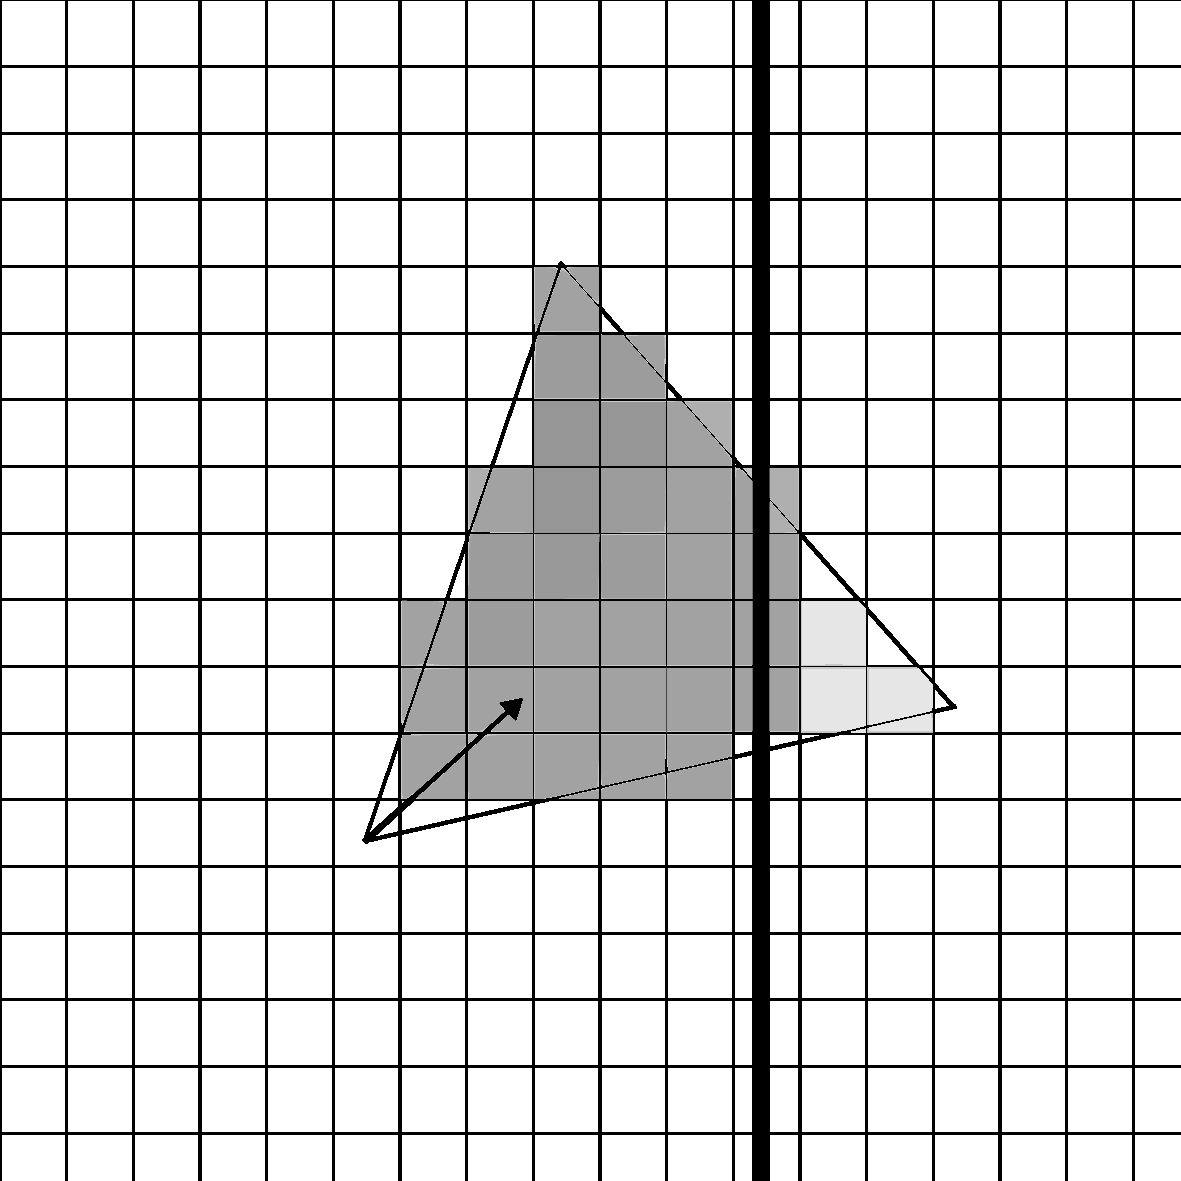
\includegraphics[width=0.5\textwidth, trim = 100 100 70 80, clip]{figures/room_type_update.pdf}
  \caption[Visualization of Room-Type-Map update]{The cells updated in the Room-Type-Map using the image taken at the robot position marked with the arrow, light gray cells are later ignored for being behind a wall and outside the room}
  \label{fig:room_type_update}
\end{figure}

Also to be considered is that not all cells visible in an image have to be of the same room type. The connection between classification result and room type probability of the cell based on the classified image is given by the following formula: 
\begin{equation}
P(R_{c}|I_{t},\mathbf{x}_{t}) = \begin{cases}\sum_{R_{I_{t} }} P(R_{I_{t} }|I_t) \; P(R_{c}|R_{I_{t}})  & if \;cell \; c \; visible\\P(R_{c}) & else\end{cases}
\end{equation}

$P(R_{c}|R_{I_{t}})$ is the probability of the room type of a cell $c$ given the room type mainly shown in the image $R_{I_{t}}$. The combinations form a $|\mathbf{R}|$x$|\mathbf{R}|$ matrix. The diagonal elements, where $R_{c} = R_{I_{t}}$, are to a parameter $V_{eq}$. Instead of presuming no prior knowledge and making all other values equal, prior knowledge is gathered to get better mapping results. The off-diagonal elements are weighted based on how related the two room types are. How much two room types are related is estimated using Divisi2, a library for extraction of information from commonsense databases, and the ConceptNet4 commonsense knowledge base. %TODO: references?

\subsection{Doorway Mapping}

The doorway mapping inserts and updates the poses of doorways in the semantic room map, using the result of the doorway detection. The result of the doorway detection is a set of doorway proposal poses in the coordinate frame of the robot. These proposal poses are transformed into the map frames of the particles. If no already found doorway is within a threshold distance to a proposal pose, a new doorway is added into the map. Otherwise the best fitting doorway, selected based on distance and orientation, is updated. This is show in figure \ref{fig:door_mapping}. A running average filter is used to estimate the true doorway pose. Due to the orientation constraint of doorway detections doorways are always facing out of the room.  
\begin{figure}[h]
\centering
  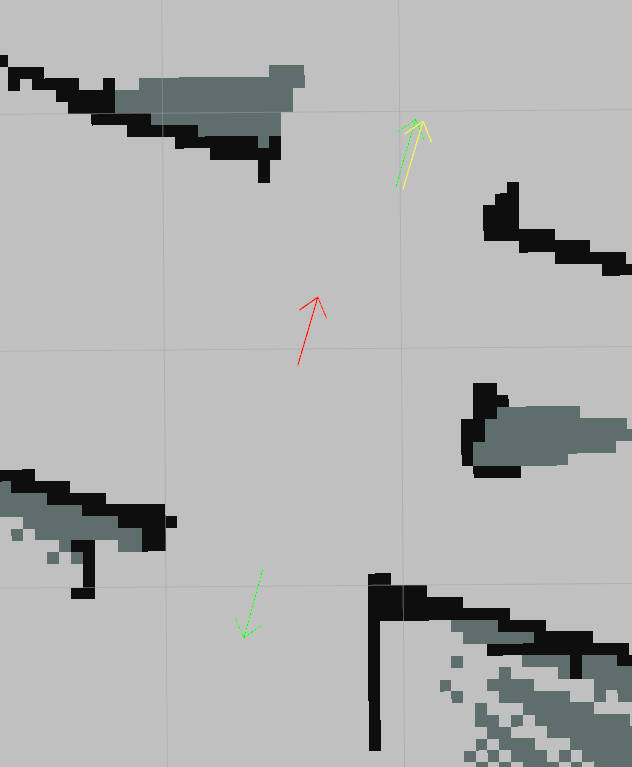
\includegraphics[width=0.5\textwidth]{figures/door_mapping.png}
  \caption[Doorway mapping example]{Doorway mapping example: The red arrow is the current robot pose, the green arrows are already found doorways, the yellow arrow is the result of the door detection, which is used to update the pose of the nearby doorway and the blue circle marks the area, which had to be free of doorways for a doorway to be added} 
  \label{fig:door_mapping}
\end{figure}

\subsection{Object-Probability-Map Estimation}

This subsection describes how the information in the different types of maps of a room are put together to obtain an estimation of the object probability at all locations in the room. This includes the estimation of the room type in location only seen by the LIDAR, the estimation of the object probabilities based on the Room-Type-Map and the combination of those estimates with the Object-Map. The Object-Probability-Map contains no information not already present in another map, therefore this map is only created when needed and only for the best particle and the searched object type. 

\subsubsection{Estimation of room types in locations only seen by the LIDAR}

The LIDAR has a field of view of 240°, while the RGBD-camera has a horizontal field of view of only 58°. This can lead to areas, which were only seen by the LIDAR. An example is shown in figure \ref{fig:seen}. 
\begin{figure}[h]
\centering
  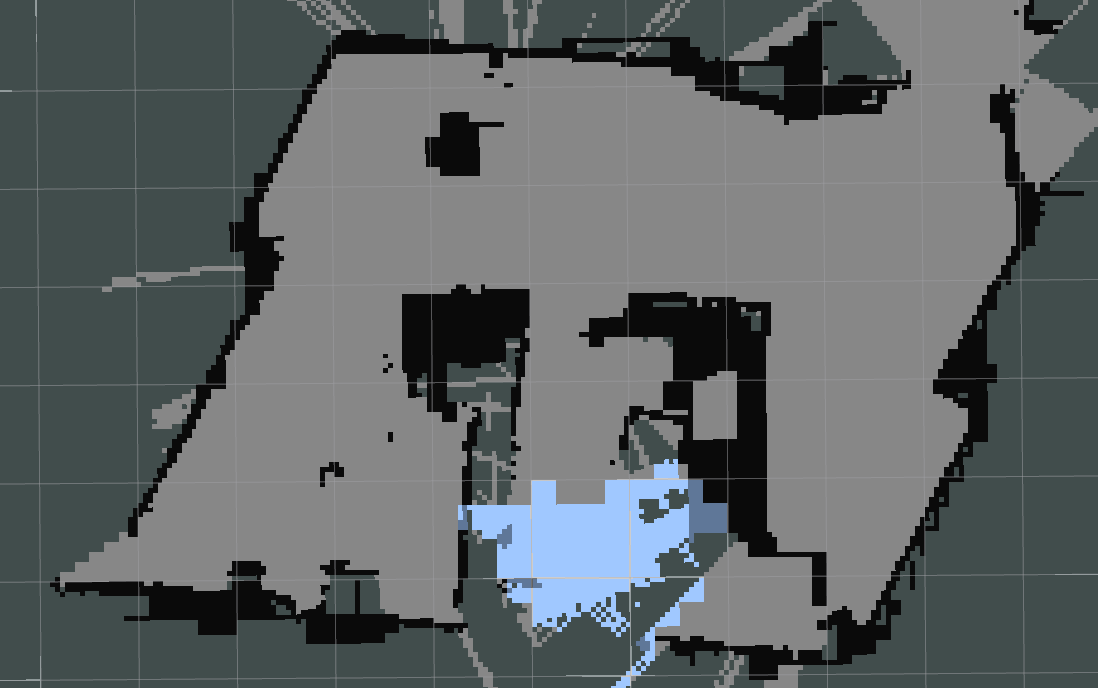
\includegraphics[width=0.8\textwidth, clip]{figures/seen.png}
  \caption[Areas only seen by LIDAR]{An explored room, light areas were only seen by the LIDAR}
  \label{fig:seen}
\end{figure}
Those cells are considered as possible object locations and are therefore of interest. Cells neither seen by the camera nor the LIDAR are ignored. The room type distribution in those areas is estimated based on the average room type distribution $P_{avg}(R_c|I_{1:t}, \mathbf{x}_{1:t})$ in the room and the room type distribution  of the neighborhood. This is done using a two dimensional Gaussian kernel $G(\Delta x, \Delta y)$, as can be seen in the following formula:
\begin{equation}
 P(R_{c}|I_{1:t}, \mathbf{x}_{1:t})= \sum_{c_2} \begin{cases} G(\Delta x, \Delta y)P(R_{c_2}|I_{1:t}, \mathbf{x}_{1:t}) & if\; c_2 \;was \; seen \;by\;camera \\ G(\Delta x, \Delta y) P_{avg}(R_c|I_{1:t}, \mathbf{x}_{1:t}) & else \end{cases}
\end{equation}


\subsubsection{Object probabilities based on the room type map}

As already described there exists a correlation between the room type of an area and the objects located in this area. This correlation is captured in the matrix K, which contains the probability of an object $o$ being in an image showing room type $r$. In a first step another matrix $K_{r,o}^*$ has to be calculated containing the probability of an object of type $o$ being in a grid cell of room type $r$. Assuming an object does not occupy multiple cells and $N_v$ cells being visible in an typical image of the dataset, the following formula is derived:
\begin{equation}
 K_{r,o}^*= 1-(1-K_{r,o})^{\frac{1}{N_v}}
\end{equation}

The probability of an object of the searched object type being in a cell based on the probability distribution of the room type of the cell $P(O_{R,c}^{o}|I_{1:t}, \mathbf{x}_{1:t})$ can be calculated with: 
\begin{equation}
 P(O_{R,c}^{o}|I_{1:t}, \mathbf{x}_{1:t})= \sum_{R_{c}}P(R_{c}|I_{1:t}, \mathbf{x}_{1:t})P(O_{R,c}^{o}|R_c)=\sum_{R_{c}}P(R_{c}|I_{1:t}, \mathbf{x}_{1:t})K_{R_{c},o}^*
\end{equation}

This calculation uses the assumption that the room type is independent of the z-coordinate of a cell, so the 2D Room-Type-Map is sufficient.

\subsubsection{Object probabilities based on all information}

In a last step the information in the Object-Map is combined with the object probabilities estimated based on the Room-Type-Map. This is done using the following formula:
\begin{equation}
 P(Obj_{c}^{o}|I_{1:t}, \mathbf{x}_{1:t})=\frac{1}{Z}P(O_{R,c}^{o}|I_{1:t}, \mathbf{x}_{1:t})P(O_{c}^{o}|I_{1:t}, \mathbf{x}_{1:t})
\end{equation}

$Z$ is a normalization term, as $P(Obj_{c}^{o}|I_{1:t}, \mathbf{x}_{1:t}) + P(\neg Obj_{c}^{o}|I_{1:t}, \mathbf{x}_{1:t}) = 1$ and can be calculated with:
\begin{equation}
 Z=P(O_{R,c}^{o}|I_{1:t}, \mathbf{x}_{1:t})P(O_{c}^{o}|I_{1:t}, \mathbf{x}_{1:t})+P(\neg O_{R,c}^{o}|I_{1:t}, \mathbf{x}_{1:t})P(\neg O_{c}^{o}|I_{1:t}, \mathbf{x}_{1:t})
\end{equation}

Some post-processing is done on the Object-Probability-Map. The probabilities of cells assumed to be outside the room are set to zero. These cells are in areas never seen by the RGBD-camera or the LIDAR or in areas behind doorways. Also probabilities in free space are set to zero. For every other cell a minimum probability is set, which is half value of the room type based probability. 

\subsection{Topological Mapping and Room Transitioning}

The topological map consists of nodes for every room, which contain the semantic room maps and condensed information for the high-level planning based on the semantic room maps. It also contains edges, where each edge corresponds to a doorway and holds information about which rooms are connected and the pose of the connecting doorway in both rooms. The topological mapping is responsible for the creation of this graphical structure, including the initialization of new room maps, the localization in the topological map and the handling of room transitions. 

When a new doorway is found a new node is inserted into the graph with an edge connecting the node of the current room and the new node. An empty semantic room map is assigned to the new node. In this map the newly detected doorway is inserted to have a valid connection between the two rooms with corresponding doorway poses in both room maps. The doorway in the new room has the same coordinates as in the current room, but the opposite orientation to meet the convention of doorways always facing out of the room. In this work environments are assumed to have no loops, meaning there is only one way into a room given a starting room. Therefore the room behind a newly found doorway cannot be already discovered. 

When a doorway is passed the semantic room map has to be switched. A doorway is passed if the robot is more than a threshold distance in front of the doorway and therefore in the next room. The threshold is marked with a blue line in the left image in Figure \ref{fig:doors}. The threshold is important to achieve a hysteresis and avoid unstable behavior at the doorway. In a first step the mapping in the old room is stopped. Then the mapping in the new room is set up. If the room was never visited before, the specified number of particles are generated with empty maps. Otherwise the best particle, including its maps, is multiplied. In a next step the particles are set to meaningful poses. Therefore the poses of the particles in the old room's particle filter are transformed into the new room's coordinate frame with
\begin{equation}
 \mathbf{P_{new}}=P_{D_{new}}T_{flip}P_{D_{old}}^{-1}\mathbf{P_{old}}
\end{equation}

$\mathbf{P_{old}}$ and $\mathbf{P_{new}}$ are the particle pose in the old and new room coordinate frames, $P_{D_{old}}$ and $P_{D_{new}}$ are the poses of the doorway in the old and new room and $T_{flip}$ is a 180° rotation matrix. The rotation is necessary as the doorway poses have an opposite orientation. After that all particles except the best one in the old rooms particle filter are discarded, as those particles are not meaningful when the robot returns to the room. In the last step the mapping in the new room is started. Figure \ref{fig:doors} shows the map before and after a doorway passing. The maps contain also space in the other room. This is necessary for navigation through the doorway. In the search planning space behind a doorway is ignored.

\begin{figure}[h]
\centering
  \subfloat[Room before doorway passing]{{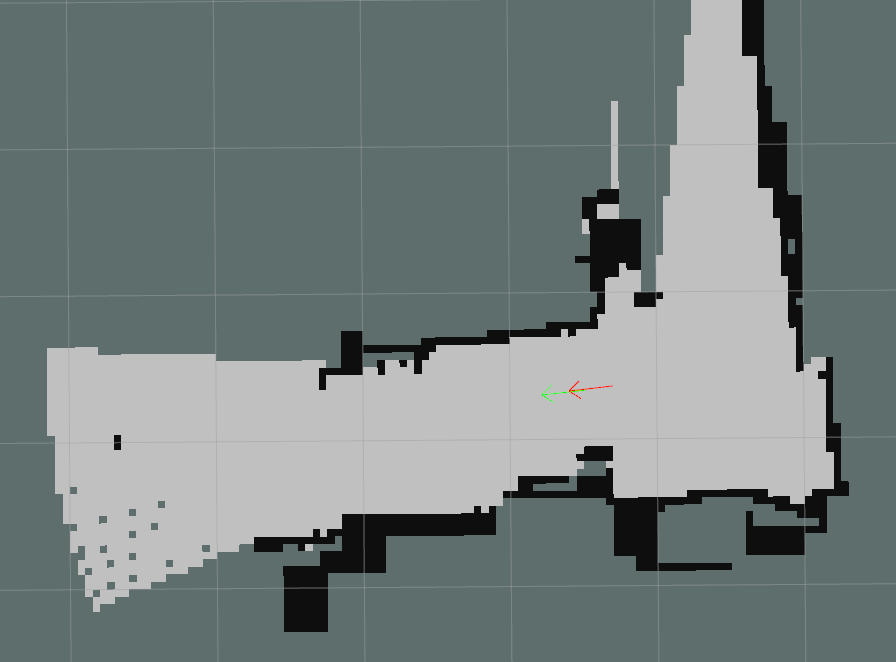
\includegraphics[width=0.45\textwidth, trim = 0 20 0 25, clip]{figures/door_gang.png} }}%
  \qquad
  \subfloat[Room after doorway passing]{{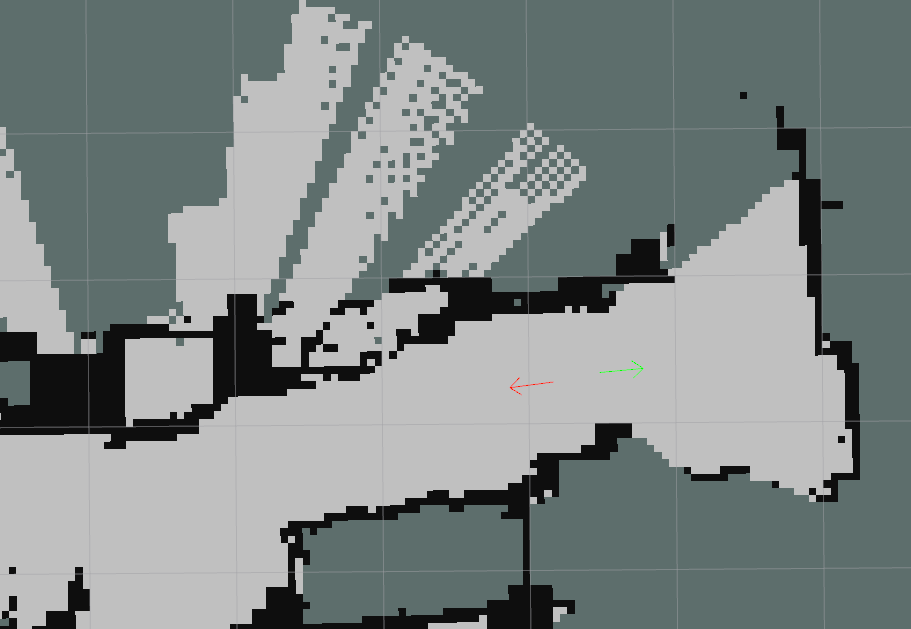
\includegraphics[width=0.45\textwidth]{figures/door_wz.png} }}%
  \caption[Doorway passing]{Doorway passing}%
  \label{fig:doors}
\end{figure}

\subsection{High-Level Room Information Generation}

For the high level planner to work the information in the semantic room maps has to be condensed into easier to used room attributes. These are
\begin{itemize}
 \item the total probability of an object of the searched object type being in the room
 \item the time needed to completely search the room
 \item the expected value of the time the robot searches in the room until an object of searched type is found or the room is completely searched 
 \item the time to traverse the room for all doorway pairs
 \item the time to leave the room for all doorways
\end{itemize}

The time needed for exploration is ignored, as it is hard to estimate and this way an incentive for exploration over searching in unlikely rooms is added. Another incentive for exploration is given by setting the object probabilities of unvisited rooms to very high values and the search times to very low values. This is done to encourage the robot to peek into rooms. Peeking into a room is a desirable behavior as it takes relatively little time and gives the robot much more information about the environment. 

\subsubsection{Total object probability in a room r $\mathbf{P_r(o)}$}

A searched object being in a room is the complementary event of no cell within the room containing the searched object and therefore can be calculated with:
\begin{equation}
 P_r(o)=P(Obj^o|I_{1:t}, \mathbf{x}_{1:t})=1-\Big(\prod_{c \in \mathbf{C_r}} (1-P(Obj_{c}^{o}|I_{1:t}, \mathbf{x}_{1:t}))\Big) 
\end{equation} 

Three types of cells within a room $\mathbf{C_r}$ have to be distinguished. There are the explored cells $\mathbf{C_{r,ex}}$, whose object probabilities are known. In not fully explored rooms also not explored cells, lying in unexplored areas of the room, have to be considered. The number of unexplored cells is estimated with:
\begin{equation}
 N_{unex} = \begin{cases} 0 & if \;room\; explored \\ max(N_{room}-|\mathbf{\mathbf{C_{r,ex}}}|, N_{min}) & else \end{cases}
\end{equation}
$N_{room}$ is a basic estimate of the size of an unexplored room and $N_{min}$ is a minimal number of unexplored cells in a not explored room. The object probability in those cells is estimated based on the average room type probability distribution $P(R_{avg})$. For the calculation of $P(Obj_{unex}^o)$ the correlation matrix between room type and object, $K^*$, is used:
\begin{equation}
 P(Obj_{unex}^o) = \sum_{R_{avg}}P(R_{avg})P(Obj_{unex}^o|R_{avg}) = \sum_{R_{avg}}P(R_{avg})K_{R_{avg},Obj_{unex}^o}^*
\end{equation}
The third type of cells are technically not within the room. Those are cells in so far undiscovered adjacent rooms. To avoid the addition of uncertain rooms into the topological map those are considered to be part of another room during probability calculation. The expected number of those cells $N_{undis}$ is estimated with:
\begin{equation}
 N_{undis}=\begin{cases} 0 & if \;room\; explored \\ max\Big(\sum_{R_{avg}}P(R_{avg})N_{adj}(R_{avg})-N_{r,dis},0\Big)N_r & else \end{cases}
\end{equation} 

$N_{adj}(R_{avg})$ is the average number of adjacent rooms for a room of type $R_{avg}$. Based on results presented in activeobjectsearchgutmapplanphd.pdf $N_{adj}(corridor)$ is set to 6 and $N_{adj}(R)$ is 1.2 for all other room types. The number of already discovered adjacent rooms $N_{r,dis}$ has to be subtracted and obviously the number of undiscovered adjacent rooms cannot be smaller than zero. The probability of the object being in one of those cells $P(Obj_{undis}^o)$ is calculated assuming a equally distributed room type probability distribution in the undiscovered room. %TODO: activeobjectsearchgutmapplanphd.pdf austauschen

Putting all together the following formula is obtained:
\begin{multline}
 P_r(o)=1-\Big(\prod_{c \in \mathbf{C_{r,ex}}} (1-P(Obj_{c}^{o}|I_{1:t}, \mathbf{x}_{1:t}))\Big)
 \\(1-P(Obj_{unex}^o))^{N_{unex}}(1-P(Obj_{undis}^o))^{N_{undis}} 
\end{multline} 

\subsubsection{Time needed to completely search room r $\mathbf{T_r}$}

The time needed to search a room is difficult to estimate, as it not only depends on the room but also on what the search planner is doing and how well the navigation works. As the generation of a lot of test data is impossible a minimalistic model is used. The number of occupied cells in the 2D map $|\mathbf{C_{occ2d}}|$ has a high correlation with the search time. A high number means many possible object locations and also many obstacles, which slow down robot movement. Therefore the time needed to completely search a room is the number of occupied cells in the 2D map within the room times a parameter $T_c$ found in test runs. Similar to the calculation of the total object probability unexplored areas in the room have to be taken into account. This is done using a basic estimated for the search time in an unexplored room $T_{room}$ and a minimum time needed for searching in unexplored areas in the room $T_{min}$. This results in
\begin{equation}
 T_r = \begin{cases} |\mathbf{C_{occ2d}}|T_c & if \;room\; explored \\ max(T_{room}, |\mathbf{C_{occ2d}}|T_c+T_{min}) & else \end{cases}
\end{equation}

\subsubsection{Expected value of time spent searching in room r $\mathbf{E_r(o)}$}

The expected value of time spent searching in a room also take into consideration that a searched object might be found and the search can be stopped earlier. The expected value is calculated with
\begin{equation}
 E_r(o) = \int_{0}^\infty f_r^o(t)\cdot t\cdot dt
\end{equation}

The search ends if the object is found or the room is completely searched. Therefore the probability distribution of ending the search over time $f_r(t)$ is
\begin{equation}
 f_r^o(t)=(1-P_r(o))\delta(T_r)+f_{find,r}^o(t)
\end{equation}
with $f_{find,r}^o(t)$ being the probability distribution over time for finding the object, which has to fulfill 
\begin{equation}
 \int_{0}^\infty f_{find,r}^o(t)\cdot dt = P_r(o)
\end{equation}
and
\begin{equation}
 f_{find,r}^o(t) = 0 \;\; \forall \; t < 0, t \geq T_r
\end{equation}

The estimation of $f_{find,r}^o(t)$ is done by discretization of time. To calculate the probability of finding the object in a time step $[T_{i-1},T_i)$ the object probabilities of all cells in the room are sorted and assigned to the time steps in decreasing order. The probability of finding the object in a certain time step $[T_{i-1},T_i)$, $P_i$, is then calculated with
\begin{equation}
 P_{i}=\prod_{j=1}^{i-1}(1-P_{j}) \cdot (1-\prod_{c \in \mathbf{C_i}}(1-P(Obj_{c}^{o}|I_{1:t}, \mathbf{x}_{1:t}))
\end{equation}
This model was chosen as it takes into account the distribution of object probabilities in the room and the decreasing probability of finding an object due to the objective of the search planner. The estimated search time is then 
\begin{equation}
 E_r(o)=\sum_i P_iT_i+(1-P_r(o))T_r 
\end{equation}

\subsubsection{Movement times}

In the high-level planning the time spent on moving into the next room to search has to be taken into account. The time needed to drive to a target room is split into the time needed to leave the starting room and the times needed to traverse rooms on the way. In this thesis the time it takes to drive from A to B is estimated by the distance between A and B multiplied with an average velocity. So for every pair of doorways in the room the estimated movement time is calculated based on their distance. The time to leave a room depends on the location of the robot, which is not known when planning in the future. Therefore an assumption is made that the robot is in the middle of the room, which is the center of mass of all free cells. For every doorway a time needed to leave the room is calculated based on the distance of the center of the room to the doorway.